% !TEX root = ../00_thesis.tex

\begin{figure}
	\centering
	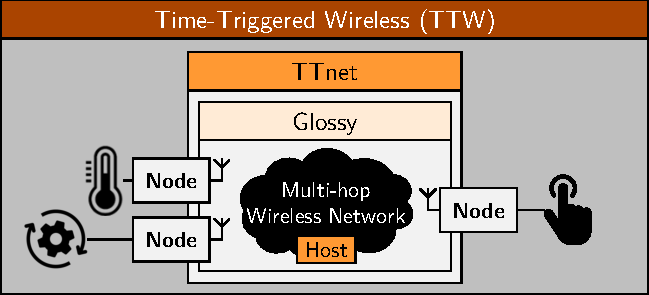
\includegraphics[scale=1]{ttw_overview}
	\caption{Overview of \TTW.
		\capt{Nodes execute distributed \CPS applications. They communicate over a multi-hop wireless network using Glossy floods~\cite{ferrari2011Glossy}.
		Communication is organized in \TTnet rounds~(\cref{fig:ttnet}) which are controlled by a central host (running on one of the nodes).
		\TTW is a global scheduler for the entire system: it co-schedules the execution time of all tasks and messages in order to reduce the end-to-end latency of applications and meet short deadlines.}
	}
	\label{fig:ttw_overview}
\end{figure}


\section{Overview of \TTW}
\label{sec:ttw_overview}

We first present \TTnet, a network stack based on synchronous transmissions (\ST), which serves as communication backbone for our solution~(\cref{subsec:ttnet}). We then introduce the concepts of \TTW~(\cref{subsec:ttw_concepts}), a system-wide scheduler built atop \TTnet to realize a wireless \CPS solution meeting the requirements described above.

\subsection{The \TTnet Communication Backbone}
\label{subsec:ttnet}

We consider a set of nodes connected by a wireless multi-hop network~(\cref{fig:ttw_overview}).
Each node is a low-power embedded device, typically battery-powered, with limited computational resources such as memory or processing power.
These devices collectively implement distributed applications (\eg closed-loop control). These applications are composed of multiple tasks and messages; the tasks are executed locally by the nodes; the messages are exchanged over the multi-hop wireless network.
In low-power wireless \CPS, a significant part of the energy is consumed by wireless communication. Thus, to minimize the energy consumption, we group messages into communication rounds, \ie time intervals where all nodes turn their radio on and communicate.
Each round is composed of dedicated time slots where nodes communicates using Glossy, a flooding protocol which delivers packets with a probability above 99.9\,\%~\cite{ferrari2011Glossy}.
The system is controlled centrally by a node called the host, which sends commands at the beginning of each round in a special slot called beacon.
Physically, one of the nodes plays the role of the host.
We call this network stack \TTnet~(\cref{fig:ttnet}).


\begin{figure}
	\centering
	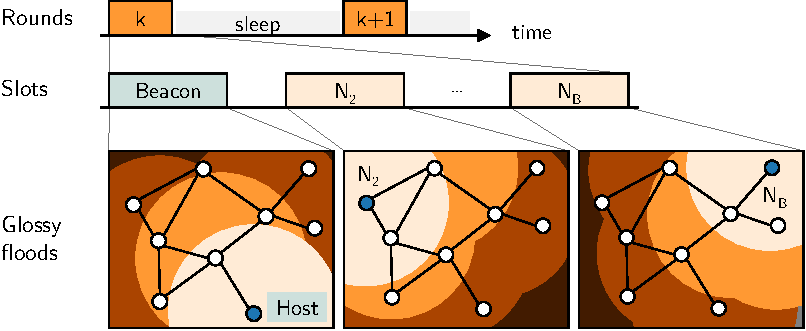
\includegraphics[scale=1]{ttnet}
	\caption{The \TTnet network stack.
	\capt
	\TTnet concept of round-based communication using Glossy floods is inspired by the Low-power Wireless Bus (LWB)~\cite{ferrari2012LWB}; this design has several benefits:%
}
\begin{itemize}

	\item
	It is based on Glossy, which has been proven to be highly reliable and energy efficient~(\cite{schuss2017Competition,lim2017Competition,escobar-molero2019Improving}).

	\squarepar{%}
		\item
		Glossy provides sub-microsecond time synchronization across the network~\cite{ferrari2011Glossy}, which is instrumental to achieve \feature{Timeliness} and \feature{Reliability}.%
	}

	\item
	The flooding process in Glossy is independent of the network state; thus it creates a virtual single-hop network where each node can communicate with every other node in bounded time. As a result, network stacks like LWB or \TTnet can be scheduled like a shared bus.

	\squarepar{%}
		\item
		As messages are flooded in the entire network, unicast multicast and broadcast are equivalent: for a given payload, the transmission time only depends on the network diameter (the maximal hop distance between nodes).

		\item
		Thanks to its stateless flooding logic, Glossy inherently supports \feature{Mobility}.%
	}

\end{itemize}

Despite these benefits, LWB or \TTnet alone cannot meet all the requirements of wireless \CPS. In particular, one must account for the scheduling of distributed tasks in order to provide end-to-end timing guarantees (\feature{Timeliness}).
\linebreak
This motivates the design of \TTW, a real-time scheduler for the \TTnet stack.

% ------------------------------------------------------------------------------
\subsection{Building-up \TTW}
\label{subsec:ttw_concepts}

The \TTnet is the communication backbone of \TTW.
Building on that structure, we design \TTW, a real-time scheduler for the entire wireless \CPS.
\linebreak
\TTW is based on four key concepts.

\begin{description}

	\item [Global co-scheduling]
	In order to minimize the achievable end-to-end latency, \TTW co-schedules the task executions and message transmissions, similarly to the state-of-the-art for wired protocols (\eg~\cite{craciunas2016Combined,zhang2014Task}).
	Moreover, the round-based design of \TTnet demands to integrates the communication rounds to the schedules. The allocation of messages to communication rounds is similar to a bin-packing problem~\cite{wikipedia2019BinPacking}.
	Combining pin-packing with traditional task-and-message co-scheduling approaches is non trivial~(\cref{sec:single_mode}).

	The resulting problem is a complex optimization that cannot be solved online, even less in a low-power setting.
	Therefore, \TTW statically synthesizes the schedule of all tasks, messages, and rounds to meet real-time constraints, minimize end-to-end latency, and minimize the energy consumed for communication.
	The schedule is synthesized by solving an MILP (mixed integer linear programming) formulation.

	\squarepar{%}
		\item[Static schedules]
		Since \TTW relies on static scheduling, we distribute the schedules at deployment time to limit the communication overhead at runtime, thus optimizing energy efficiency.
		Each node stores its own schedule information, thereby trading-off memory utilization with energy consumption; this significantly improves the \feature{Efficiency} of the system.%
	}

	\item[Multiple operation modes]
	The obvious drawback of using static schedules is that the system always execute the same schedule, compromising \feature{Adaptability}.
	\TTW mitigates this problem by using the traditional concept of operation modes~\cite{fohler1993changing}:
	Multiple schedules are computed offline and stored in the nodes' memory. The system can switch at runtime between different modes, thereby recovering some degree of \feature{Adaptability}.



	\item[Runtime control]
	At the beginning of each round, the host sends a beacon, which is used to control the system execution at runtime.
	A beacon contains the current round \id, the mode \id, and a trigger bit \SB used in the mode change procedure~(\cref{sec:modeChanges}).

	Thanks to the distributed schedule information, it is sufficient for any node to receive a single beacon to retrieve the system state (\ie the phase of the schedule given by the round \id) and therefore know
	% \begin{itemize}
		% \linebreak
		% \inlineitem
		(i)~which message to send in which slot, and
		% \\
		% \inlineitem
		(ii)~when to wake up for the next communication round.
		% \\
	% \end{itemize}
	If a node does not receive the beacon, it does not participate in the round. Hence, even if nodes miss some control information, they do not initiate a communication in a slot allocated to another node, thus guaranteeing conflict-free communication~(\feature{Reliability}).

\end{description}

\squarepar{%}
	By globally optimizing the entire system schedule, \TTW can meet tight end-to-end deadlines (tens of \ms) while minimizing the energy spent for wireless communication, thus addressing the \feature{Timeliness} and \feature{Efficiency} requirements.
	The runtime control based on beacons provides \feature{Reliability}, while switching between multiple operation modes at runtime offers some degree of \feature{Adaptability}.
	Finally, \feature{Mobility} is supported by design thanks to the stateless logic of Glossy~\cite{ferrari2011Glossy}, the underlying communication primitive used by \TTW.%
}

\begin{remark}
	\TTW combines offline scheduling and online decisions whereas \DRP~(\cref{ch:drp}), by contrast, does everything online.
	Hence, \TTW trades the flexibility of execution of the distributed application tasks for short latency and fast mode changes.
\end{remark}
